\documentclass[conference,a4paper]{IEEEtran}
\usepackage{cite,amsmath,amssymb,graphicx,booktabs,algorithmic,url}
\usepackage{tikz}
\usetikzlibrary{arrows.meta,positioning,shapes.geometric}

\newcommand{\TBD}{\textit{TBD}}
\newcommand{\Planned}{\textit{Planned}}

\begin{document}

\title{A Data Quality-Aware Smart Parking AI Agent for Arrival-Time-Oriented On-Street Parking Availability Prediction}

\author{\IEEEauthorblockN{Author Name}
\IEEEauthorblockA{Department of Computer Science and Engineering\\
National Chung Hsing University\\
Taichung, Taiwan\\
author@example.com}}

\maketitle

\begin{abstract}
Real-time on-street parking displays often report available spaces at query time, yet drivers frequently encounter full segments upon arrival. Existing parking prediction studies largely target off-street garages or isolated forecasting models, while New Taipei City's historical JSONL parking feeds still require full-scale verification of spatial coverage, temporal granularity, and data quality. To address this discrepancy, this study proposes a data quality-aware Smart Parking AI Agent that autonomously plans data tasks, selects tools, enforces quality gates, and produces traceable, risk-aware top-$k$ recommendations conditioned on estimated arrival time. The proposed architecture integrates an API/data connector layer, a quality gate, past-only feature construction, Persistence, Historical Median, and tree-based forecasting models, domain capacity rules, and an Agent Orchestrator equipped with retry/replan and human-review fallbacks. Evaluation is designed around a strict chronological 60/20/20 split (training, validation, and test) comparing against Persistence and Historical Median baselines using MAE, RMSE, PR-AUC, Brier Score, and Top-$k$ Success. In preliminary prototype verification, a sampled notebook achieved an MAE of approximately 7.12 spaces and nine unit tests passed across connector, quality gate, baseline, and orchestrator modules; full-dataset quality auditing, formal recommendation evaluation, full-scale training, and deployment remain planned and unverified.
\end{abstract}

\begin{IEEEkeywords}
smart parking, AI agent, on-street parking, arrival-time forecasting, data quality, risk calibration, intelligent transportation systems
\end{IEEEkeywords}

\section{Introduction}

\subsection{Background and Motivation}
Drivers searching for on-street parking frequently rely on real-time occupancy feeds that reflect conditions at query time rather than at estimated arrival time. In dense urban areas such as New Taipei City, Taiwan, turnover on roadside parking segments can invalidate instantaneous vacancy counts within minutes. Consequently, decision support must shift from reporting current availability to predicting segment occupancy conditioned on estimated arrival time and quantifying the risk that a segment becomes full before arrival.

\subsection{Identified Research Gaps}
This work distinguishes two complementary gaps derived from problem analysis:
\begin{enumerate}
    \item \textbf{Empirical Data Gap:} Historical New Taipei City on-street JSONL records (covering May 1, 2025 to November 2, 2026) require full-scale empirical verification of segment coverage, sampling granularity, reporting latency, duplicate entries, and abnormal status codes before complex predictive models can be trusted.
    \item \textbf{Project-Specific Integration Gap:} Reliable driver recommendations require jointly integrating multi-source data quality checks, arrival-time full-occupancy risk estimation, API failure replanning, and traceable top-$k$ decision explanations into a unified workflow.
\end{enumerate}

\subsection{Research Hypotheses and Justification of an AI Agent}
We formulate three research hypotheses ($H_1$--$H_3$) to be tested in formal experiments:
\begin{itemize}
    \item \textbf{$H_1$ (Arrival-Time Forecasting):} Past-only temporal and horizon-conditioned features improve arrival-time availability accuracy over Persistence and Historical Median baselines under chronological evaluation.
    \item \textbf{$H_2$ (Risk-Aware Recommendation):} Combining point forecasts with calibrated full-occupancy probability and data-quality penalties increases Top-$k$ recommendation success over proximity-only or uncalibrated point-based ranking.
    \item \textbf{$H_3$ (Agent Orchestration Value):} An autonomous AI Agent outperforms a rigid static pipeline when facing real-world operational faults.
\end{itemize}
Specifically, a simple deterministic pipeline is preferable whenever data sources are stable and execution steps are fixed. An AI Agent becomes necessary only when dynamic tool selection, API timeout or error recovery (retry and replanning), data freshness gating, and low-confidence abstention via human-in-the-loop review are required to prevent unreliable recommendations.

\subsection{Contributions and Organization}
The main contributions of this study are: (1) an arrival-time-oriented formulation anchored to a strict data contract and past-only feature construction; (2) explicit per-observation data quality assessment coupled with calibrated full-occupancy risk scoring; and (3) a replan-capable Smart Parking AI Agent with verifiable execution logic and clear separation between verified prototype results and planned evaluations. The remainder of this paper reviews related work (Section~\ref{sec:related}), establishes domain design principles (Section~\ref{sec:domain}), details the proposed AI Agent architecture and algorithm (Section~\ref{sec:method}), specifies the data contract and experimental protocol (Section~\ref{sec:data}), and summarizes current prototype status and planned work (Section~\ref{sec:status}).

\section{Related Work}\label{sec:related}

To balance artificial intelligence techniques with parking domain knowledge, related research is examined across predictive modeling, uncertainty calibration, and operational parking constraints.

\subsection{Parking Availability Prediction and Domain Studies}
Classic parking availability studies analyze off-street parking lots and sensor-equipped facilities, such as the Birmingham car park benchmark~\cite{stolfi2017,stolfi2017uci}. Existing literature spans statistical and duration models, spatiotemporal deep learning architectures, Bayesian uncertainty estimation, and digital twin frameworks. In parallel, nonlinear ensemble methods such as random forests~\cite{breiman2001} and gradient boosted trees (\textsc{XGBoost})~\cite{chen2016} provide strong tabular baselines when engineered with lagged occupancy, rolling statistics, and calendar features.

\subsection{Uncertainty Calibration and Transferability Limitations}
For decision support under full-occupancy risk, raw regression or classification scores must be mapped to well-calibrated probabilities using methods such as Platt scaling~\cite{platt1999} or isotonic regression~\cite{zadrozny2002}. Table~\ref{tab:literature} summarizes representative method families and highlights key barriers when transferring prior approaches directly to New Taipei City on-street parking: heterogeneous sensing infrastructure, legacy or off-street-centric datasets, absence of explicit API-failure replanning, and lack of empirical validation on New Taipei City's roadside JSONL feeds.

\begin{table}[!t]
\caption{Comparison of Related Method Families and Transferability Gaps}
\label{tab:literature}
\centering
\scriptsize
\setlength{\tabcolsep}{3pt}
\begin{tabular}{p{1.6cm}p{1.55cm}p{1.65cm}p{2.2cm}}
\toprule
\textbf{Method Family} & \textbf{Target Setting} & \textbf{Quality / Risk} & \textbf{Limitation for New Taipei On-Street} \\
\midrule
Statistical / Duration & Off-street / fixed sensor & Limited drift handling & Assumes stationary or uniform intervals \\
Tree Ensembles \cite{breiman2001,chen2016} & Tabular / urban lots & Point prediction by default & Requires past-only leak guards and external calibration \\
Spatiotemporal Deep Models & Dense sensor networks & Often uncalibrated & High data sensitivity; lacks New Taipei validation \\
Bayesian / Digital Twin & Simulation / instrumented sites & Explicit uncertainty & Heavy infrastructure assumptions; high deployment cost \\
Proposed AI Agent & New Taipei on-street JSONL & Per-record quality gate + \cite{platt1999,zadrozny2002} & Handles API faults, freshness, and traceable Top-$k$ \\
\bottomrule
\end{tabular}
\end{table}

\section{Domain Analysis and Design Principles}\label{sec:domain}

\subsection{Five Core Design Mindsets}
Five domain principles govern the system design:
\begin{enumerate}
    \item \textbf{Data quality precedes model complexity:} Auditing duplicates, missingness, and reporting latency is mandatory before training complex models.
    \item \textbf{Model formulation must match prediction horizon:} Features and error targets must reflect the arrival horizon $h = t_a - t$.
    \item \textbf{Preserve spatial and operational semantics:} On-street roadside segments behave differently from gated off-street parking lots and must not be conflated.
    \item \textbf{Beat simple baselines first:} Any candidate model must demonstrably outperform Persistence and Historical Median under identical splits.
    \item \textbf{Uncertainty is a decision input:} Calibrated full-occupancy risk and observation quality directly inform ranking and abstention rather than serving only as offline diagnostics.
\end{enumerate}

\subsection{Three Technical Controversies and Adopted Stances}
\begin{itemize}
    \item \textbf{Simple vs.\ Deep Spatiotemporal Models:} Rather than assuming deep models are superior, tree-based and baseline models are compared against complex architectures under identical chronological splits.
    \item \textbf{Unified vs.\ Segment-Specific Models:} A shared global model enriched with segment attributes is evaluated first and compared systematically against segment-specific models.
    \item \textbf{Point Prediction vs.\ Risk-Aware Recommendation:} We combine point vacancy forecasts with separately calibrated full-occupancy probabilities rather than misrepresenting a single heuristic score as full uncertainty decomposition.
\end{itemize}

\section{Proposed Smart Parking AI Agent}\label{sec:method}

\subsection{System Architecture and Decision Workflow}
Fig.~\ref{fig:architecture} illustrates the end-to-end eight-stage Agent architecture and decision workflow: (1) \textbf{User / GIS} supplies the destination and estimated arrival time; (2) \textbf{Planner} decomposes the query and manages a replan budget $K$; (3) \textbf{Tool Selection \& Connectors} invoke historical JSONL or real-time API sources; (4) \textbf{Quality Gate} verifies schema validity, abnormal status codes, and freshness (triggering \textit{Retry / Replan} upon failure); (5) \textbf{Past-only Features} constructs leakage-free lag and horizon features; (6) \textbf{Model / Baseline} predicts remaining spaces with capacity bounds; (7) \textbf{Risk Rules \& Ranking} computes calibrated full-occupancy risk and Top-$k$ scores; and (8) \textbf{Explain / Verify} checks output confidence, returning traceable recommendations or escalating to \textbf{Human Review} when confidence is insufficient.

\begin{figure}[!t]
\centering
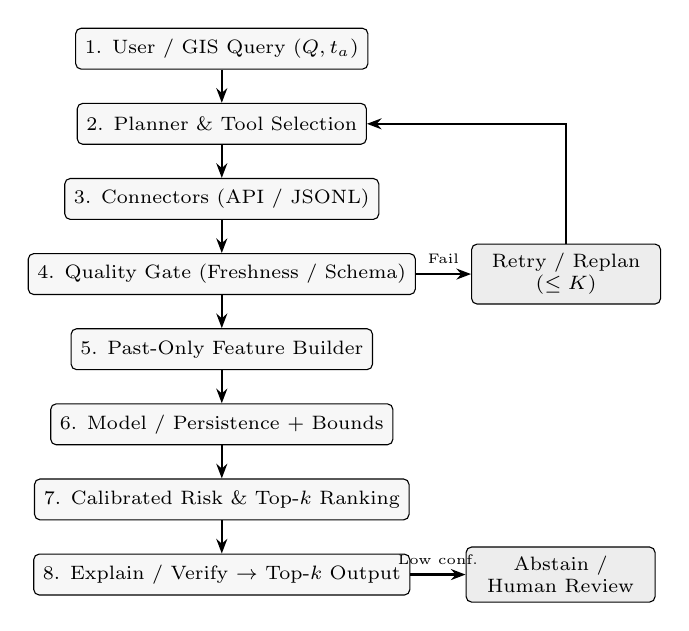
\begin{tikzpicture}[
    node distance=4.2mm and 6mm,
    box/.style={draw, rounded corners=2pt, align=center, font=\scriptsize, minimum width=3.3cm, minimum height=5.2mm, fill=gray!6},
    decision/.style={draw, rounded corners=2pt, align=center, font=\scriptsize, minimum width=2.4cm, minimum height=5.0mm, fill=gray!14},
    arrow/.style={-{Stealth[scale=0.8]}, thick}
]
\node[box] (user) {1. User / GIS Query $(Q, t_a)$};
\node[box, below=of user] (plan) {2. Planner \& Tool Selection};
\node[box, below=of plan] (conn) {3. Connectors (API / JSONL)};
\node[box, below=of conn] (gate) {4. Quality Gate (Freshness / Schema)};
\node[box, below=of gate] (feat) {5. Past-Only Feature Builder};
\node[box, below=of feat] (model) {6. Model / Persistence + Bounds};
\node[box, below=of model] (risk) {7. Calibrated Risk \& Top-$k$ Ranking};
\node[box, below=of risk] (verify) {8. Explain / Verify $\rightarrow$ Top-$k$ Output};

\node[decision, right=7mm of gate] (retry) {Retry / Replan\\($\leq K$)};
\node[decision, right=7mm of verify] (human) {Abstain /\\Human Review};

\draw[arrow] (user) -- (plan);
\draw[arrow] (plan) -- (conn);
\draw[arrow] (conn) -- (gate);
\draw[arrow] (gate) -- (feat);
\draw[arrow] (feat) -- (model);
\draw[arrow] (model) -- (risk);
\draw[arrow] (risk) -- (verify);

\draw[arrow] (gate.east) -- node[above, font=\tiny]{Fail} (retry.west);
\draw[arrow] (retry.north) |- (plan.east);
\draw[arrow] (verify.east) -- node[above, font=\tiny]{Low conf.} (human.west);
\end{tikzpicture}
\caption{Proposed eight-stage Smart Parking AI Agent architecture with retry/replan and human-review loops.}
\label{fig:architecture}
\end{figure}

\subsection{Problem Formulation and Quality-Aware Scoring}
Let $y_{s,t}$ denote available spaces on road segment $s$ at query time $t$, and $C_s$ its verified capacity. Given estimated arrival time $t_a > t$, the prediction horizon is
\begin{equation}
h = t_a - t.
\label{eq:horizon}
\end{equation}
Using only features $\mathbf{x}_{s,t}$ strictly observable at or before $t$, the bounded forecast is
\begin{equation}
\hat{y}_{s,t_a} = \operatorname{clip}\!\left(f_\theta(\mathbf{x}_{s,t}, h),\, 0,\, C_s\right),
\label{eq:forecast}
\end{equation}
where the Persistence baseline sets $\hat{y}^{\mathrm{pers}}_{s,t_a} = y_{s,t_{\mathrm{last}}}$. For each candidate observation $o$, a per-observation quality vector $o.\mathrm{quality}$ evaluates freshness, completeness, and status validity, yielding a scalar quality score $q_s \in [0,1]$:
\begin{equation}
q_s = \sum_{j=1}^{m} w_j z_{s,j}, \quad \sum_{j=1}^{m} w_j = 1, \quad w_j \geq 0.
\end{equation}
To balance proximity against occupancy and quality uncertainty, eligible segments are ranked using
\begin{equation}
R_s = \alpha(1 - p_{\mathrm{full},s}) - \beta d_s - \gamma(1 - q_s),
\label{eq:rank}
\end{equation}
where $p_{\mathrm{full},s}$ is the calibrated probability of zero available spaces at arrival, $d_s$ is normalized walking distance, and $\alpha, \beta, \gamma \geq 0$ are tuned on validation data.

\subsection{Agent Execution Algorithm and Quality-Propagation Fix}
Fig.~\ref{fig:algorithm} details the Agent decision procedure. Crucially, line~21 computes \texttt{forecast.risk} using each candidate's own observation quality $o.\mathrm{quality}$ inside the per-observation loop, resolving an implementation defect (C1) in which a single trailing candidate's quality could inadvertently overwrite risk estimates across all candidates.

\begin{figure}[!t]
\centering
\begin{minipage}{0.96\columnwidth}
\footnotesize
\begin{algorithmic}[1]
\REQUIRE Query $Q$, tool registry $T$, max replans $K$
\ENSURE Ranked Top-$k$ $R$ or human-review request
\STATE $\text{req} \leftarrow \textsc{Parse}(Q)$
\STATE $\text{plan} \leftarrow \textsc{Planner}(\text{req}, T.\text{caps})$
\STATE $r \leftarrow 0$; $\text{obs} \leftarrow \emptyset$
\WHILE{$r \leq K$}
    \STATE $\text{raw} \leftarrow \textsc{RunConnectors}(\text{plan})$
    \STATE $(\text{ok}, \text{obs}) \leftarrow \textsc{QualityGate}(\text{raw})$
    \IF{$\text{ok}$}
        \STATE \textbf{break}
    \ENDIF
    \STATE $r \leftarrow r + 1$; $\text{plan} \leftarrow \textsc{Replan}(\text{plan}, \text{raw})$
\ENDWHILE
\IF{$\text{obs} = \emptyset$}
    \RETURN $\textsc{HumanReview}(\text{``No valid data''})$
\ENDIF
\STATE $\text{preds} \leftarrow \emptyset$
\FOR{each $o \in \text{obs}$}
    \STATE $\mathbf{x} \leftarrow \textsc{PastFeatures}(o, \text{req}.t_a)$
    \STATE $m \leftarrow \textsc{SelectModel}(o.\text{type}, \text{req}.h)$
    \STATE $f \leftarrow m.\textsc{Predict}(\mathbf{x})$ if $m$ else $\textsc{Persist}(\mathbf{x})$
    \STATE $f \leftarrow \textsc{BoundCap}(f, o.\text{spaces})$
    \STATE $f.\text{risk} \leftarrow \textsc{EstRisk}(f, o.\text{quality})$ \COMMENT{C1 fix}
    \STATE Append $f$ to $\text{preds}$
\ENDFOR
\STATE $R \leftarrow \textsc{CalibrateAndRank}(\text{preds})$
\IF{$\textsc{LowConfidence}(R)$}
    \RETURN $\textsc{HumanReview}(R.\text{evidence})$
\ENDIF
\RETURN $R$
\end{algorithmic}
\end{minipage}
\caption{Smart Parking AI Agent execution algorithm incorporating retry/replan, past-only feature enforcement, per-observation risk estimation (C1), and human-review abstention.}
\label{fig:algorithm}
\end{figure}

\section{Data Contract, Quality Audit, and Experimental Protocol}\label{sec:data}

\subsection{New Taipei City Data Contract and UCI Audit Findings}
The primary dataset comprises New Taipei City on-street historical JSONL records spanning May 1, 2025 to November 2, 2026. To prevent temporal leakage and duplicated keys, the data contract defines the composite primary key $(\text{source}, \text{segment\_id}, \text{observed\_at})$ normalized to \texttt{Asia/Taipei}, enforces strictly past-only feature construction relative to query availability time, and matches ground truth using the nearest valid post-arrival observation.

As an empirical sanity check on real-world parking feeds prior to full New Taipei auditing, our quality pipeline was validated on the UCI Parking Birmingham benchmark~\cite{stolfi2017uci}. The audit identified \textbf{216 duplicate records} and systematic \textbf{overnight reporting gaps}, demonstrating that equal-spaced, gap-free time series cannot be assumed without explicit quality gating. Table~\ref{tab:data} summarizes the dataset contract and audit status.

\begin{table}[!t]
\caption{Dataset Contract and Audit Status}
\label{tab:data}
\centering
\scriptsize
\setlength{\tabcolsep}{3.5pt}
\begin{tabular}{p{2.1cm}p{3.6cm}l}
\toprule
\textbf{Dataset / Attribute} & \textbf{Specification / Finding} & \textbf{Status} \\
\midrule
New Taipei On-Street & JSONL, 2025/05/01--2026/11/02 & Contracted \\
Primary Key & $(\text{source}, \text{segment\_id}, \text{observed\_at})$ & Enforced \\
Records / Segments & \TBD & \Planned \\
Missing Rate / Latency & \TBD & \Planned \\
UCI Birmingham~\cite{stolfi2017uci} & 216 duplicates; overnight gaps & Verified \\
\bottomrule
\end{tabular}
\end{table}

\subsection{Chronological Split, Metrics, and Go/No-Go Thresholds}
All experiments follow a strict chronological \textbf{60\% Train / 20\% Validation / 20\% Test} split with zero cross-partition overlap. Forecasting accuracy is measured by $\mathrm{MAE}$ and $\mathrm{RMSE}$ against \textbf{Persistence} and \textbf{Historical Median} baselines across candidate horizons (e.g., 5, 15, 30, and 60 minutes). Full-occupancy probabilities are calibrated on the validation split via Platt scaling~\cite{platt1999} or isotonic regression~\cite{zadrozny2002} and evaluated using \textbf{PR-AUC} and \textbf{Brier Score}. End-to-end utility is measured via \textbf{Top-$k$ Success} ($\mathrm{Hit@}k$), reporting label coverage separately so missing ground truth is never misclassified as success or failure. Candidate deployment requires satisfying predefined \textbf{Go/No-Go} gates, including at least a \textbf{5\% MAE reduction} relative to Persistence and at least a \textbf{5\% gain in Top-3 Success}.

\section{Implementation Status, Preliminary Findings, and Roadmap}\label{sec:status}

To maintain strict scientific rigor, verified prototype artifacts are explicitly separated from planned full-scale experiments (Table~\ref{tab:status}). At the current proposal milestone:
\begin{itemize}
    \item \textbf{Verified Prototype:} Four core prototype modules (\texttt{Connector}, \texttt{Quality Gate}, \texttt{Baseline}, and \texttt{Agent Orchestrator}) have been implemented with \textbf{9 passing unit tests}. A sampled notebook prototype achieved an MAE of approximately \textbf{7.12 spaces} (prototype-only, non-exhaustive sample).
    \item \textbf{Planned / Unverified Work:} Full-scale auditing of the New Taipei City JSONL archive, full-dataset model training and hyperparameter tuning, probability calibration verification, formal Top-$k$ recommendation benchmarking, and production deployment remain scheduled for final-project execution.
\end{itemize}

\begin{table}[!t]
\caption{Verification Status and Planned Experimental Benchmarks}
\label{tab:status}
\centering
\scriptsize
\setlength{\tabcolsep}{3pt}
\begin{tabular}{p{1.85cm}p{2.45cm}p{1.85cm}l}
\toprule
\textbf{Item} & \textbf{Scope / Baseline} & \textbf{Metric / Result} & \textbf{Status} \\
\midrule
Prototype Tests & Connector, Gate, Agent & 9 / 9 pass & Verified \\
Sampled Notebook & Prototype sample & MAE $\approx 7.12$ & Prototype \\
Full Data Audit & New Taipei (25/05--26/11) & Coverage, latency & \Planned \\
Forecasting & Persist.\ vs.\ Median vs.\ Trees & MAE ($\geq 5\%$ gain) & \Planned \\
Risk Calibration & Platt / Isotonic & PR-AUC, Brier & \Planned \\
Top-$k$ Utility & Quality-aware vs.\ prox. & Top-3 ($\geq 5\%$ gain) & \Planned \\
\bottomrule
\end{tabular}
\end{table}

\section{Conclusion}
This paper presents a data quality-aware Smart Parking AI Agent designed for arrival-time-oriented on-street parking prediction and risk-aware top-$k$ recommendation in New Taipei City. Grounded in explicit data contracts, past-only feature safeguards, per-observation quality gating, and retry/replan plus human-review fallbacks, the framework bridges real-world data imperfections and driver decision support. Current prototype tests and UCI benchmark audits confirm the necessity of quality-first orchestration, while full-dataset validation and formal Go/No-Go benchmarking will be completed in subsequent experiments.

\bibliographystyle{IEEEtran}
\bibliography{references}

\end{document}
